\documentclass[10pt]{article}

\usepackage{amsmath, amssymb, mathtools}
\usepackage{tikz}
\usepackage[margin=1.5cm]{geometry}

\DeclareFontFamily{U}{wncy}{}
\DeclareFontShape{U}{wncy}{m}{n}{<->wncyr10}{}
\DeclareSymbolFont{mcy}{U}{wncy}{m}{n}
\DeclareMathSymbol{\Sh}{\mathord}{mcy}{"58}

\input pdfmsym
\input prettyprint
\input ../infi3/preamble

\pdfmsymsetscalefactor{10}
\initpps

\newfunc{fourier}{\mathcal{F}}({})
\newfunc{ifourier}{\mathcal{F}^{-1}}({})
\newfunc{cis}{{\rm cis}}({})
\newfunc{Sha}{\Sh}({})

\parskip=3pt plus 3pt minus 3pt

\def\pmat#1{\begin{pmatrix} #1 \end{pmatrix}}
\def\@ppmathcount{\thesection.\thepp@mathcount}

\begin{document}

\font\bigbf = cmbx12 scaled 2000
\barcolorbox{220, 255, 220}{0, 130, 0}{80, 200, 80}{
    \leftskip=0pt plus 1fill \rightskip=\leftskip
    {\bigbf Fourier Analysis of Signals}

    \medskip
    \textit{Image Processing, Bar Ilan Winter Semester $2022-2023$}

    \textit{Ari Feiglin}
}

\section{The Fourier Transformation}

First, we begin with a crucial first definition:

\begin{defn*}

    Given a function $f\colon\bR\longvarrightarrow\bR$, its \ppemph{Fourier Transform} is:
    \[ \fourierof{f(x)}(u) = \int_{-\infty}^\infty f(x)\cdot e^{-i2\pi ux}\,dx \]
    That is, $\fourierof{f}$ is a function mapping real numbers to complex numbers.
    (The complex unit is $i$: $i^2=-1$).

\end{defn*}

Another way we can think of this is as $\fourier$ being a function mapping functions $f\colon\bR\longvarrightarrow\bR$ to functions $\bR\longvarrightarrow\bC$.
Not every function has a Fourier transformation, but for the sake of this summary, it doesn't matter.

Now what's crucial about the Fourier Transform is that it is \emph{invertible}, that is there exists an inverse transformation $\ifourier$ such that
\[ \ifourierof{\fourierof{f(x)}}=f(x),\quad \fourierof{\ifourierof{F(u)}} = F(u) \]
And this inverse transformation is given by:
\[ \ifourierof{F(u)}(x) = \int_{-\infty}^\infty F(u)\cdot e^{i2\pi ux}\,du \]

Let's take a moment to understand what this means.
Suppose we have a function $f(x)$ and we take its Fourier transformation $F(u)=\fourierof{f(x)}(u)$.
Then by taking the inverse Fourier transformation of $F$ we get that:
\[ f(x) = \ifourierof{F(u)}(x) = \int_{-\infty}^\infty F(u) e^{i2\pi ux}\,du \]
Now recall that $F(u)$ is a complex number, so it can be written as $A_u\cdot e^{i\theta_u}$, and this becomes:
\[ f(x) = \int_{-\infty}^\infty A_u\cdot e^{i(x\cdot 2\pi u + \theta_u)}\,du \]
And we know that functions of the form $e^{i\theta}$ is a sinusoidal wave:
\[ e^{i\theta} = \cis(\theta) = \sin(\theta) + i\cos(\theta) \]
And so
\[ A_ue^{i(x\cdot 2\pi u + \theta_u)} = A_u\cis(x\cdot 2\pi u + \theta_u) \]
this is a sinusoidal wave of \emph{frequency} $u$, \emph{phase} $\theta_u$, and \emph{amplitude} $A_u$.
Recall that the \emph{phase} of a complex number is its argument, ie. the phase of $re^{i\theta}$ is $\theta$ and its \emph{amplitude} is its magnitude ($r$).
What this means is that we can write $f$ as the integral of sinusoidal waves whose frequency is given by $u$, and the phase and amplitude are the phase and amplitude of $F(u)$.

So the Fourier Transform of a function $f$ gives us a decomposition of $f$ into sinusoidal waves.

Furthermore, we can extend the definition of the Fourier Transformation to multivariable functions quite elegantly:

\newpage
\begin{defn*}

    Given a function $f(x_1,\dots,x_n)\colon\bR^n\longvarrightarrow\bR$, we define its \emph{Fourier Transform} to be:
    \[ \fourierof{f(x_1,\dots,x_n)}(u_1,\dots,u_n) = \int_{-\infty}^\infty\cdots\int_{-\infty}^\infty f(x_1,\dots,x_n)\cdot e^{-i2\pi(u_1x_1+\cdots+u_nx_n)}\,dx_1\cdots dx_n \]
    Or more compactly:
    \[ \fourierof{f(\vec x)}(\vec u) = \int_{\bR^n} f(\vec x)\cdot e^{-i2\pi \vec u\cdot\vec x}\,d\vec x \]
    where the product $\vec u\cdot\vec x$ is the \ppemph{dot product} of two vectors.

    Notice that $\fourierof{f(\vec x)}$ is a function $\bR^n\longvarrightarrow\bC$.

\end{defn*}

Similarly, the inverse multidimensional Fourier Transformation of $F(\vec u)$ is:
\[ \ifourierof{F(\vec u)}(\vec x) = \int_{\bR^n} F(\vec u)\cdot e^{i2\pi\vec u\cdot\vec x}\,d\vec u \]
The significance of this is similar to that of the single dimension case: this decomposes $f(\vec x)$ into multidimensional sinusoidal waves whose amplitude and phase are given by $F(\vec u)$.
But here sinusoidal waves are multidimensional, they are of the form:
\[ A_u e^{i(u_1x_1+\cdots+u_nx_n+\theta_u)} = A_u\cis\bigl(u_1x_1+\cdots+u_nx_n+\theta_u\bigr) \]
(this is multidimensional since there are $n$ inputs: $x_1,\dots,x_n$).
The sinusoidal waves in multiple dimensions are a bit more complicated, but fundamentally are very similar to the one dimension case.

It may be worthwhile to explicitly write the Fourier Transform and its inverse for two dimensions:
\[ \fourierof{f(x,y)}(u,v) = \int_{-\infty}^\infty\int_{-\infty}^\infty f(x,y)\cdot e^{-i2\pi(ux+vy)}\,dxdy \]
and
\[ \ifourierof{F(u,v)}(x,y) = \int_{-\infty}^\infty\int_{-\infty}^\infty F(u,v)\cdot e^{i2\pi(ux+vy)}\,dudv \]

Let's now discuss a few important traits of the Fourier Transform.

\benum
    \item The Fourier Transformation is \emph{linear}: for every two functions $f,g\colon\bR^n\longvarrightarrow\bR$:
    \[ \fourierof{f(\vec x) + g(\vec x)}(\vec u) = \fourierof{f(\vec x)}(\vec u) + \fourierof{g(\vec x)}(\vec u) \]
    and for every $\alpha\in\bR$:
    \[ \fourierof{\alpha f(\vec x)}(\vec u) = \alpha\fourierof{f(\vec x)}(\vec u) \]

    \item The Fourier Transformation also \emph{scales}: for $\alpha_1,\dots,\alpha_n$ real numbers:
    \[ \fourierof{f(\alpha_1 x_1,\dots,\alpha_n x_n)}(u_1,\dots,u_n) = \frac1{\abs{\alpha_1\cdots\alpha_n}}\fourierof{f(x_1,\dots,x_n)}\parens{\frac{u_1}{\alpha_1},\dots,\frac{u_n}{\alpha_n}} \]
    In two dimensions, given $\alpha$ and $\beta$ this becomes:
    \[ \fourierof{f(\alpha x,\beta y)}(u,v) = \frac1{\abs{\alpha\beta}}\fourierof{f(x,y)}\parens{\frac u\alpha, \frac v\beta} \]

    \item In two dimensions, the Fourier Transformation of the rotation of $f(x,y)$ is equal to the rotation of the Fourier Transformation of $f(x,y)$ with the same angle.

    \item If the Fourier Transformation of $f(\vec x)$ is $F(\vec u)$ then the Fourier Transformation of $f(\vec x-\vec x_0)$ is:
    \[ \fourierof{f(\vec x-\vec x_0)}(\vec u) = \int_{\bR^n} f(\vec x-\vec x_0)\cdot e^{-i2\pi(\vec u\cdot\vec x)}\,d\vec x = \int_{\bR^n} f(\vec x)\cdot e^{-i2\pi(\vec u\cdot(\vec x+\vec x_0))}\,d\vec x
    = e^{-i2\pi\vec u\cdot\vec x_0}\cdot F(\vec u) \]
\eenum

Finally we get the following important theorem:

\begin{thrm*}[convThrm,The\ Convolution\ Theorem]

    If $f$ and $g$ are functions, whose Fourier Transformations are $F$ and $G$ respectively, then:
    \[ \fourierof{f\ast g(x)}(u) = F(u)\cdot G(u) \]
    and
    \[ \fourierof{f(x)\cdot g(x)}(u) = F\ast G(u) \]
    where $f\ast g$ denotes the \ppemph{convolution} of $f$ and $g$.

\end{thrm*}

\section{Sampling and the Discrete Fourier Transformation}

Suppose we have a signal $f$ and we'd like to investigate it.
That is, we'd like to figure out its decomposition into frequencies, ie. its Fourier Transformation.
This is not always possible; for example, suppose we're receiving a radio signal.
We don't have the actual formula for the signal, we just have values of the signal which we've \emph{sampled} at (constant) intervals of time.

In order to understand this, we first we begin with an important mathematical object:

\begin{defn*}

    The \ppemph{Dirac Delta Function} is a mathematical object denoted $\delta(x)$ where for every real function $f$:
    \[ \int_{-\infty}^\infty f(x)\cdot\delta(x)\,dx = f(0) \]
    In multiple dimensions, the multidimensional Diract Delta Function, $\delta(\vec x)$ satisfies:
    \[ \int_{\bR^n} f(\vec x)\cdot\delta(\vec x)\,d\vec x = f(\vec 0) \]

\end{defn*}

The Dirac Delta Function allows us to sample an input signal at a specific time.

Notice that if we shift the Diract Delta Function, we get:
\[ \int_{-\infty}^\infty f(x)\cdot\delta(x-x_0)\,dx = \int_{-\infty}^\infty f(x+x_0)\cdot\delta(x)\,dx = f(0+x_0) = f(x_0) \]
And in multiple dimensions:
\[ \int_{\bR^n} f(\vec x)\cdot\delta(\vec x - \vec x_0)\,dx = f(\vec x_0) \]
Specifically, in two dimensions:
\[ \int_{-\infty}^\infty\int_{-\infty}^\infty f(x,y)\cdot\delta(x-x_0, y-y_0)\,dxdy = f(x_0, y_0) \]

As one final trait, notice that for $\alpha>0$:
\[ \int_{-\infty}^\infty f(x)\cdot\delta(\alpha x)\,dx = \frac1\alpha\int_{-\infty}^\infty f\parens{\frac x\alpha}\cdot\delta(x)\,dx = \frac1\alpha\cdot f(0) \]
and if $\alpha<0$:
\[ \int_{-\infty}^\infty f(x)\cdot\delta(\alpha x)\,dx = -\frac1\alpha\int_{-\infty}^\infty f\parens{\frac x\alpha}\cdot\delta(x)\,dx = \frac1\alpha\cdot f(0) \]
and so $\delta(\alpha x)$ acts the same as $\frac1{\abs\alpha}\delta(x)$, so we say
\[ \delta(\alpha x) = \frac1{\abs\alpha}\delta(x) \]

Notice that the Fourier Transform of the delta function is:
\[ \fourierof{\delta(\vec x)}(\vec u) = \int_{\bR^n}\delta(\vec x)\cdot e^{-2i\pi \vec u\cdot\vec x}\,d\vec x = e^{-2i\pi \vec u\cdot\vec0} = e^0 = 1 \]

This allows us to define another important function:

\begin{defn*}

    The \ppemph{Sha} function is defined as:
    \[ \Shaof x = \sum_{n=-\infty}^\infty \delta(x-n) \]

\end{defn*}

This can of course be generalized to multiple dimensions, but for the sake of this summary, we will focus on the one dimensional case.

Notice that for a real $\tau>0$:
\[ \Shaof{\frac x\tau} = \sum_{n=-\infty}^\infty \delta\parens{\frac x\tau -n} = \sum_{n=-\infty}^\infty \tau\delta\parens{x-\tau n} = \tau\sum_{n=-\infty}^\infty\delta\parens{x-\tau n} \]
Thus we can use the $\Sha$ function to \emph{sample} an input signal $f$: suppose we'd like to sample an input signal at intervals of $\tau$ units of time, that is we'd like to sample it at
times $\dots, -2\tau, -\tau, 0, \tau, 2\tau, \dots$.
Recall that the Dirac Delta Function can give us the measurement of the function at a specific time, so we define the \emph{sampled function} of $f$, to be:
\[ f_s(x) = f(x)\cdot\Shaof{\frac x\tau} \]

Suppose that $F(u)=\fourierof{f(x)}(u)$.
Recall that by \ppref{convThrm}, the Fourier Transform of a product is the convolution of the convolution of the Fourier Transforms.
Applying that here, we get that
\[ \fourierof{f_s(x)}(u) = \sum_{n=-\infty}^\infty F\parens{u-\frac n\tau} \]

Let's take a moment to understand the significance of this.
Suppose we have a signal whose Fourier Transform, $F$ looks like:

{\centering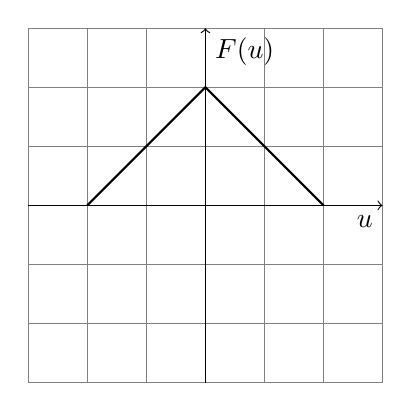
\begin{tikzpicture}[scale=1.5]
    \draw[step=0.5, color=gray, thin]
        (-1.5, 1.5) grid (1.5, -1.5);
    \draw[black, domain=-1:1, variable=\x, thick]
        plot ({\x}, {1-abs(\x)});
    \draw[black, ->]
        (0,-1.5) -- (0, 1.5) node[anchor=north west] {$F(u)$};
    \draw[black, ->]
        (-1.5, 0) -- (1.5, 0) node [anchor=north east] {$u$};
\end{tikzpicture}\par}

Then the Fourier Transform of $f_s$ becomes:

{\centering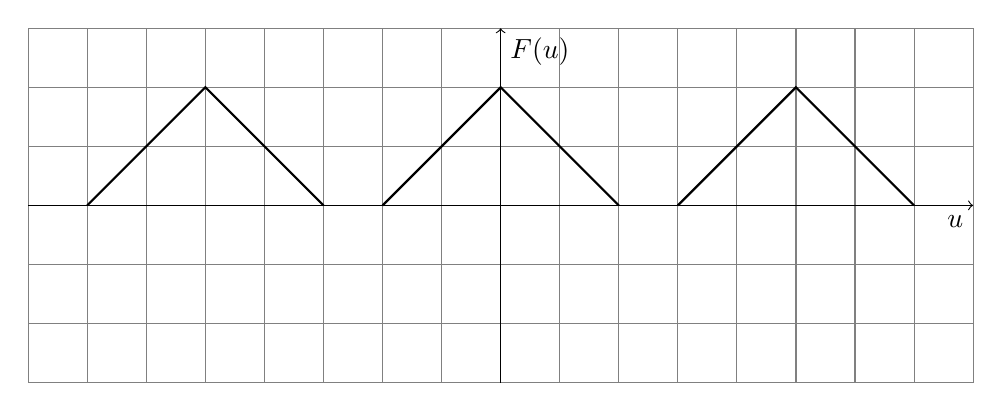
\begin{tikzpicture}[scale=1.5]
    \draw[step=0.5, color=gray, thin]
        (-4, 1.5) grid (4, -1.5);
    \foreach \i in {-2.5, 0, 2.5}{
        \draw[black, domain={\i-1}:{\i+1}, variable=\x, thick]
            plot ({\x}, {1-abs(\x-\i)});
    }
    \draw[black, ->]
        (0,-1.5) -- (0, 1.5) node[anchor=north west] {$F(u)$};
    \draw[black, ->]
        (-4, 0) -- (4, 0) node [anchor=north east] {$u$};
\end{tikzpicture}\par}

And this continues in both directions for infinity.
But this assumes that $\frac n\tau$ is spaced out enough that the $F\parens{u-\frac n\tau}$ don't overlap.
If $\tau$ is too large, and thus $\frac n\tau$ too small, we get instead something which looks like:

{\centering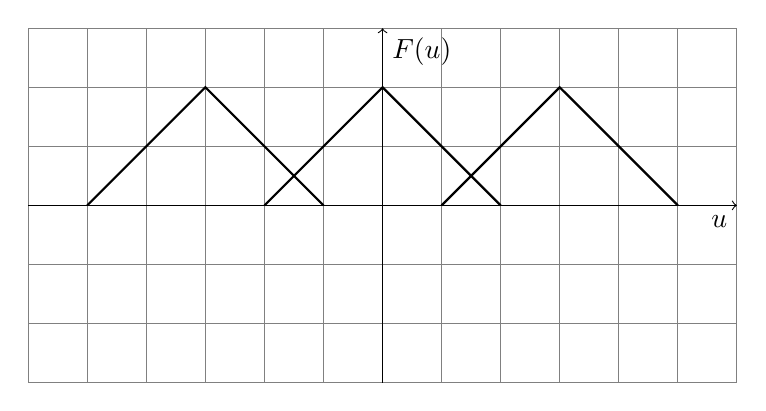
\begin{tikzpicture}[scale=1.5]
    \draw[step=0.5, color=gray, thin]
        (-3, 1.5) grid (3, -1.5);
    \foreach \i in {-1.5, 0, 1.5}{
        \draw[black, domain={\i-1}:{\i+1}, variable=\x, thick]
            plot ({\x}, {1-abs(\x-\i)});
    }
    \draw[black, ->]
        (0,-1.5) -- (0, 1.5) node[anchor=north west] {$F(u)$};
    \draw[black, ->]
        (-3, 0) -- (3, 0) node [anchor=north east] {$u$};
\end{tikzpicture}\par}

The overlaps here actually mean that the values are added up, but in any case this causes inaccuracies in our sampled Fourier Transform.
This phenomenon is called \emph{undersampling}.
But if $\tau$ is small enough, using a discrete sampling of the signal, we can reconstruct the Fourier Transform of the original signal, or at least a good approximation.
But what $\tau$ is small enough?
Suppose that largest frequency in the decomposition of $f(x)$ is $f_0$, that is for every $f_1>f_0$, $F(f_0)=0$.
Then we must have that $f_0-\frac1\tau\leq -f_0$ ($-f_0$ is the leftmost point in $F(u)$ in the sampled Fourier Transformation, and $f_0-\frac1\tau$ is the rightmost point in $F\parens{u-\frac n\tau}$),
and so

\[ 2f_0\leq\frac1\tau \implies \tau\leq\frac1{2f_0} \]
Recall that the period of the wave of frequency $f_0$ is $\frac1{f_0}$, so we must sample at least twice for each period of the wave of the highest frequency in order to sample without causing undersampling.
This maximum frequency is called the \emph{Nyquist Frequency}:

\begin{defn*}

    The \ppemph{Nyquist Frequency} of a signal $f(x)$ is the largest frequency of sampling (we sample at $\dots,-\tau,0,\tau,\dots$ where $\tau$ is the Nyquist frequency) in order to not cause undersampling.
    The Nyquist frequency is equal to $\frac1{2f_0}$ where $f_0$ is the largest frequency in the decomposition of $f(x)$ into waves (the smallest value where $F(u)=0$ afterward).

\end{defn*}

Let's now see now how we can actually find a discrete decomposition of $f(x)$.
Recall that:
\[ f_s(x) = f(x)\cdot\Shaof{\frac x\tau} = \tau\cdot\sum_{n=-\infty}^\infty f(x)\cdot\delta(x-\tau n) \]
And so we can find another formula for the Fourier Transformation of the sampled function directly using the definition of the Fourier Transformation:
\[ \fourierof{f_s(x)}(u) = \sum_{n=-\infty}^\infty\int_{-\infty}^\infty f(x)\cdot\delta(x-\tau n)\cdot e^{-2\pi ux}\,dx = \sum_{n=-\infty}^\infty f(\tau n)\cdot e^{-i2\pi u\tau n} \]
Now suppose instead of sampling an infinite number of times, we take $N$ samples at times $0,\Delta x,\dots,(N-1)\Delta x$, so $\tau=\Delta x$ and this becomes:
\[ \sum_{n=0}^{N-1} f\parens{n\cdot\Delta x}\cdot e^{-i2\pi nu\Delta x} \]
We can create a sequence $x[0],\dots,x[N-1]$ of the samples of $f(x)$, ie. $x[n]=f(n\Delta x)$.
Now suppose that we only care about sampling this Fourier Transformation at $N$ points with frequency $\Delta u$, that is we only care about $X[k]=F(k\cdot\Delta u)$, then
\[ X[k] = \sum_{n=0}^{N-1} x[n]\cdot e^{-i2\pi nk\Delta x\Delta u} \]
If we further require that $\Delta x\cdot\Delta u=\frac1N$ we get that
\[ X[k] = \sum_{n=0}^{N-1} x[n]\cdot e^{-i\frac{2\pi}Nnk} \]
This is called the \emph{Discrete Fourier Transformation} of $f$:

\begin{defn*}

    Given a signal $f$ which we sample $N$ times with frequency $\Delta x$, sampling the Fourier Transformation $N$ times with frequency $\frac1{\Delta x}$ gives:
    \[ X[k] = \sum_{n=0}^{N-1} x[n]\cdot e^{-i\frac{2\pi}Nnk},\qquad k=0,\dots,N-1 \]
    where $x[n]$ is the $n$th sample of $f(x)$ and $X[k]$ is the $k$th sample of the Fourier Transformation of $f$.

    $X$ is called the \ppemph{Discrete Fourier Transformation} (DFT) of $x$.

\end{defn*}

The \emph{inverse Discrete Fourier Transformation} (IDFT) of $X$ should not be too surprising:
\[ x[n] = \frac1N\sum_{k=0}^{N-1} X[k]\cdot e^{-i\frac{2\pi}Nnk},\qquad n=0,\dots,N-1 \]
Some conventions multiply the DFT by $\frac1N$ instead of the IDFT.
This has the benefit that $X[0]$ is equal to the average of $x[0],\dots,x[N-1]$ (as opposed to the sum), $X[0]$ is called the \emph{DC} component.

We can generalize this to more dimensions, but we do just two here:

\begin{defn*}

    Given a matrix $x[0,\dots,N-1\,;\,0,\dots,M-1]$ its \ppemph{Discrete Fourier Transformation} is:
    \[ X[u,v] = \sum_{j=0}^{M-1}\sum_{t=0}^{N-1} x[t,j]\cdot e^{-i2\pi\parens{\frac{ut}N+\frac{vj}M}},\qquad \begin{array}{l}u=0,\dots,N-1\\v=0,\dots,M-1\end{array} \]

\end{defn*}

Similarly, the \emph{inverse Discrete Fourier Transformation} of $X$ is:
\[ x[t,j] = \frac1{NM}\sum_{v=0}^{M-1}\sum_{u=0}^{N-1}X[u,v]\cdot e^{i2\pi\parens{\frac{ut}N+\frac{vj}M}},\qquad \begin{array}{l}t=0,\dots,N-1\\j=0,\dots,M-1\end{array} \]
Some conventions multiply the DFT by $\frac1{NM}$ instead of the IDFT.

Notice that in order to compute $X$, we can first find the DFT of each row of $x$ and the find the DFT of each of the columns in that new matrix (or find the DFT of the columns first, and then the rows).

What's important about the DFT is that it (and the IDFT) can be computed in $O(N\log N)$ time (as opposed to $O(N^2)$ time naively), algorithms which do this are called \emph{Fast Fourier Transform} (FFT)
algorithms.

\section{Frequency Filters}

A special type of noise in a signal is \emph{periodic noise}.
Periodic noise is of course periodic.
In order to deal with it, we use Fourier Transformations in order to find the suspect frequencies of the noise, set them to $0$ and then find the inverse Fourier Transformation of this.
This gives a signal where these suspect frequencies no longer exist, hopefully getting rid of the periodic noise.
Using FFT, this can be done with relative efficiency.
An important related function for this is \emph{FFTShift}, which takes the DFT of the signal and shifts it so that the center of the output corresponds to $X\bigl[\vec0\bigr]$; the DC component.
This makes it easier for us to see the frequencies, since the higher frequencies are at the edges, and the lower frequencies are near the center.

Also, we are mostly concerned with the amplitudes of the frequencies, so given a DFT of an image, we are more concerned with the magnitude of each complex number.
The phase of each complex number is still very important as it gives the phase of the frequency, but it's harder for us to understand how each phase affects the image.
Furthermore, since the dynamic range of the amplitudes is quite large, to us the DFT would like almost dark with a bright speck in the center (the DC component).
So we take a logarithmic scale of the DFT; $\log(1+\abs{X})$ ($\abs{X}$ since we are concerned with the amplitudes).

Another use of the Fourier Transform (and FFT) is convoluting the image.
Recall that convolutions in the image are equivalent to elementwise products in the frequency space.
So instead of convoluting an image, we can find the DFT of the image and the mask, multiply them together elementwise, and then find the IDFT of this new image.
For very large masks, this may be more efficient than convoluting the image.
More specifically: suppose we have an image $x[0,\dots,N-1\,;\,0,\dots,M-1]$ and a mask $k[0,\dots,N-1\,;\,0,\dots,M-1]$.
Suppose the DFT of $x$ is $X$ and the DFT of $k$ is $K$.
Then:
\[ x\ast k = {\rm IDFT}(X\cdot K) \]
where the product is element-wise.

Relative to frequencies, there are three types of filters:

\benum
    \item \textbf{High Pass Filters} (HPFs) are filters which preserve or amplify higher frequencies, and significantly reduce (set to $0$) lower frequencies.
    The most simple HPF is a filter $H(u,v)=0$ if $\sqrt{u^2+v^2}\leq t$ for some threshold $t$ (since $(u,v)$ corresponds to the frequency of the sinusoidal wave $\cis(ux+vy+\theta)$, which has relatively
    low frequency), and $H(u,v)=1$ if $\sqrt{u^2+v^2}>t$.
    \item \textbf{Low Pass Filters} (LPFs) are filters which preserve or amplify lower frequencies, and set higher frequencies to $0$.
    The most simple LPF is a filter is a filter $H(u,v)=1$ if $\sqrt{u^2+v^2}\leq t$ and $H(u,v)=0$ otherwise.
    \item \textbf{Bandpass Filters} (BPFs) are filters which preserve or amplify frequencies within a certain interval/band, and set other frequencies to $0$.
    The most simple BPF is a filter $H(u,v)=1$ if $t_1\leq\sqrt{u^2+v^2}\leq t_2$ for thresholds $t_1$ and $t_2$ and $H(u,v)=0$ otherwise.
\eenum

Notice that in order to approximate a discontinuity, it requires many high frequencies.
So HPFs show us areas of discontinuity (or high rates of change), which correspond closely to the edges of an image.
And since LPFs get rid of areas of high rate of change, they correspond to blurring the image.

A \textbf{High Frequency Emphasis} filter (HFE) is a filter of the form:
\[ k_0 + k_1H(u,v) \]
where $H$ is a HPF.
Its purpose is to preserve lower frequencies (which is the purpose of adding $k_0$) and emphasizes higher frequencies (the purpose of $k_1H$).
HFEs are usually used in conjunction with histogram equalization (after filtering the image, equalize the histogram).

\end{document}

